%% LyX 2.3.4.2 created this file.  For more info, see http://www.lyx.org/.
%% Do not edit unless you really know what you are doing.
\documentclass[11pt,english]{article}
\usepackage[T1]{fontenc}
\usepackage[latin9]{inputenc}
\usepackage[a4paper]{geometry}
\geometry{verbose,tmargin=2cm,bmargin=2cm,lmargin=2cm,rmargin=2cm}
\usepackage{color}
\usepackage{float}
\usepackage{amsmath}
\usepackage{graphicx}

\makeatletter

%%%%%%%%%%%%%%%%%%%%%%%%%%%%%% LyX specific LaTeX commands.
%% Because html converters don't know tabularnewline
\providecommand{\tabularnewline}{\\}

\makeatother

\usepackage{babel}
\begin{document}
\noindent \begin{flushleft}
\begin{tabular}{llr}
Mattias Villani  & \hspace{8.1cm} & Bayesian Statistics I \tabularnewline
Department of Statistics &  & \tabularnewline
Stockholm University  &  & \tabularnewline
\end{tabular}
\par\end{flushleft}

\vspace{0.3cm}

\noindent \begin{flushleft}
\begin{tabular}{l}
\multicolumn{1}{l}{\textbf{\large{}{}Computer Lab 1 }}\tabularnewline
\multicolumn{1}{l}{\rule{0.975\columnwidth}{1pt}}\tabularnewline
\multicolumn{1}{l}{You are recommended to use R for solving the labs. }\tabularnewline
\multicolumn{1}{l}{You work and submit your labs in pairs, but both of you should contribute
equally}\tabularnewline
and understand all parts of your solutions.\tabularnewline
\multicolumn{1}{l}{\texttt{\textbf{\textcolor{blue}{It is not allowed to share exact
solutions}}} with other student pairs.}\tabularnewline
Submit your solutions via Athena.\tabularnewline
\multicolumn{1}{l}{\rule{0.975\columnwidth}{1pt}}\tabularnewline
\end{tabular}
\par\end{flushleft}

{\footnotesize{}\vspace{0.5cm}
}{\footnotesize\par}
\begin{enumerate}
\item \emph{Bernoulli ... again.}\\
Let $y_{1},...,y_{n}|\theta\sim\mathrm{Bern}(\theta)$, and assume
that you have obtained a sample with $s=14$ successes in $n=20$
trials. Assume a $\mathrm{Beta}(\alpha_{0},\beta_{0})$ prior for
$\theta$ and let $\alpha_{0}=\beta_{0}=2$.

\begin{enumerate}
\item Draw random numbers from the posterior $\theta\vert y\sim\mathrm{Beta}(\alpha_{0}+s,\beta_{0}+f)$,
$y=(y_{1},\dots,y_{n}),$ and verify graphically that the posterior
mean and standard deviation converges to the true values as the number
of random draws grows large.
\item Use simulation (\texttt{nDraws = 10000}) to compute the posterior
probability $\mathrm{Pr}(\theta<0.4\vert y)$ and compare with the
exact value {[}Hint: \texttt{pbeta()}{]}.
\item Compute the posterior distribution of the log-odds $\phi=\log\frac{\theta}{1-\theta}$
by simulation (\texttt{nDraws = 10000}). {[}Hint: \texttt{hist()}
and \texttt{density()} might come in handy{]}
\end{enumerate}
\item \emph{Log-normal distribution and the Gini coefficient.}\\
Assume that you have asked 10 randomly selected persons about their
monthly income (in thousands Swedish Krona) and obtained the following
ten observations: 14, 25, 45, 25, 30, 33, 19, 50, 34 and 67. A common
model for non-negative continuous variables is the log-normal distribution.
The log-normal distribution $\log\mathcal{N}(\mu,\sigma^{2})$ has
density function
\[
p(y\vert\mu,\sigma^{2})=\frac{1}{y\cdot\sqrt{2\pi\sigma^{2}}}\exp\left[-\frac{1}{2\sigma^{2}}\left(\log y-\mu\right)^{2}\right],
\]
for $y>0$, $\mu>0$ and $\sigma^{2}>0$. The log-normal distribution
is related to the normal distribution as follows: if $y\sim\log\mathcal{N}(\mu,\sigma^{2})$
then $\log y\sim\mathcal{N}(\mu,\sigma^{2})$. Let $y_{1},...,y_{n}\vert\mu,\sigma^{2}\overset{iid}{\sim}\log\mathcal{N}(\mu,\sigma^{2})$,
where $\mu=3.5$ is assumed to be known but $\sigma^{2}$ is unknown
with non-informative prior $p(\sigma^{2})\propto1/\sigma^{2}$. The
posterior for $\sigma^{2}$ is the $Inv-\chi^{2}(n,\tau^{2})$ distribution,
where
\[
\tau^{2}=\frac{\sum_{i=1}^{n}(\log y_{i}-\mu)^{2}}{n}.
\]

\begin{enumerate}
\item Simulate $10,000$ draws from the posterior of $\sigma^{2}$ (assuming
$\mu=3.5$) and compare with the theoretical $Inv-\chi^{2}(n,\tau^{2})$
posterior distribution.
\item The most common measure of income inequality is the Gini coefficient,
$G$, where $0\leq G\leq1$. $G=0$ means a completely equal income
distribution, whereas $G=1$ means complete income inequality. See
Wikipedia for more information. It can be shown that $G=2\Phi\left(\sigma/\sqrt{2}\right)-1$
when incomes follow a $\log\mathcal{N}(\mu,\sigma^{2})$ distribution.
$\Phi(z)$ is the cumulative distribution function (CDF) for the standard
normal distribution with mean zero and unit variance. Use the posterior
draws in a) to compute the posterior distribution of the Gini coefficient
$G$ for the current data set.
\item Use the posterior draws from b) to compute a 95\% equal tail credible
interval for $G$. An 95\% equal tail interval $(a,b)$ cuts off $2.5\%$
percent of the posterior probability mass to the left of $a$, and
$2.5\%$ to the right of $b$. Also, do a kernel density estimate
of the posterior of $G$ using the \texttt{density} function in R
with default settings, and use that kernel density estimate to compute
a 95\% Highest Posterior Density interval for $G$. Compare the two
intervals.
\end{enumerate}
\item Bayesian inference for the concentration parameter in the von Mises
distribution. This exercise is concerned with directional data. The
point is to show you that the posterior distribution for somewhat
non-standard models can be obtained by plotting it over a grid of
values. The wind direction was measured once a month at a given location.
The data were recorded in degrees, and the measurements for the first
ten months were
\[
(40,303,326,285,296,314,20,308,299,296),
\]
where North is located at zero degrees. To fit with Wikipedias description
of probability distributions for circular data we convert the data
into radians $-\pi\leq y\leq\pi$ . The $10$ observations in radians
are 
\[
(-2.44,2.14,2.54,1.83,2.02,2.33,-2.79,2.23,2.07,2.02),
\]
where South is now at a radian of $0$ and North is at $\pm\pi$.
See Figure 1 for a visualization of the data in radians. Assume that
these data points are independent observations following the von Mises
distribution
\[
p(y\vert\mu,\kappa)=\frac{\exp\left[\kappa\cdot\cos(y-\mu)\right]}{2\pi I_{0}(\kappa)},\;-\pi\leq y\leq\pi,
\]
where $I_{0}(\kappa)$ is the modified Bessel function of the first
kind of order zero {[}see \texttt{?besselI} in R{]}. The parameter
$\mu$ ($-\pi\leq\mu\leq\pi$) is the mean direction and $\kappa>0$
is called the concentration parameter. Large $\kappa$ gives a small
variance around $\mu$, and vice versa. Assume that $\mu$ is known
to be $2.39$. Let $\kappa\sim\mathrm{Exponential}(\lambda=1)$ a
priori, where $\lambda$ is the rate parameter of the exponential
distribution (so that the mean is $1/\lambda$).

\begin{enumerate}
\item Plot the posterior distribution of $\kappa$ for the wind direction
data over a fine grid of $\kappa$ values.
\item Find the (approximate) posterior mode of $\kappa$ from the information
in a).
\end{enumerate}
{\footnotesize{}\vspace{0.5cm}
}{\footnotesize\par}
\end{enumerate}
\begin{figure}[H]
\begin{centering}
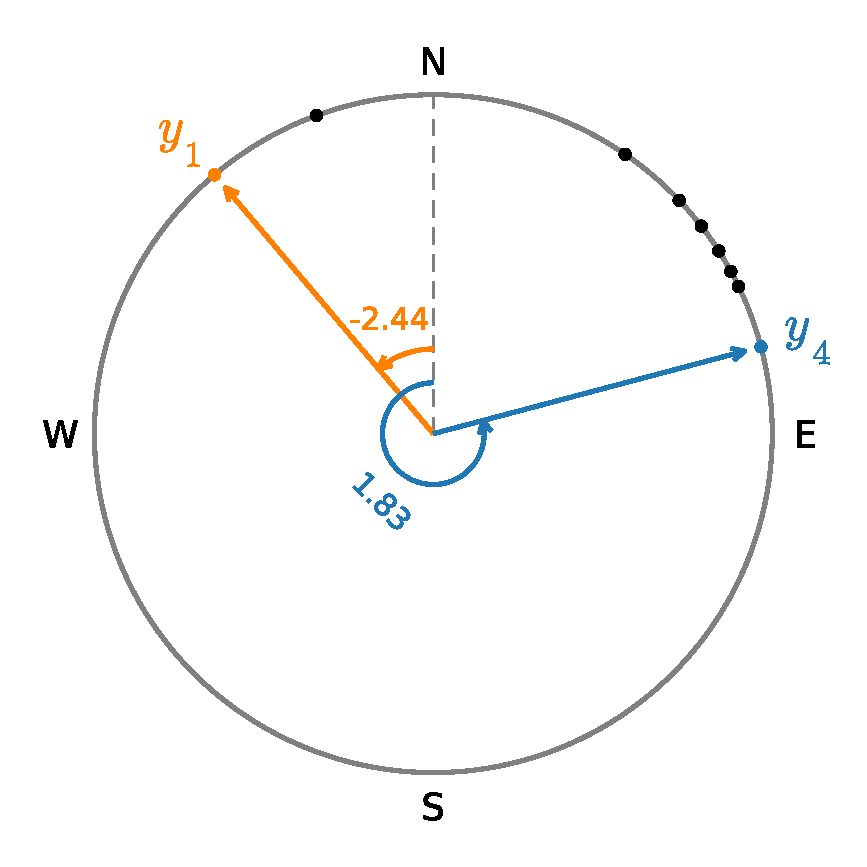
\includegraphics[scale=0.5]{directionaldata}
\par\end{centering}
\caption{The wind direction data $y\in(-\pi,\pi)$. South is at $y=0$ radians
and North is at $y=\pm\pi$.}
\end{figure}

\end{document}
